\section{Normalizing a Multi-BPM Map}
Even if you don't consider \textbf{ever} mapping/modding a multi-BPM map, you will still find this concept useful. So unless you fully understand \textbf{Normalizing}, do not skip this chapter!

\subsection{The idea of "Normalization"}
Normalization in this context means adding SV lines over BPM lines in order to force the map to run at a \textbf{constant scroll speed}, that is, \textbf{1.0x}.

\subsection{Normalizing a simple Beatmap}

\subfile{../part_3/figs/norm_fig1.tex}

This is one of the more common cases of multi-BPM that you'll come across, where the song itself will change BPMs in a simplistic way. \newline
Take note of the bracketed value beside each BPM (eg. 300\textbf{(1.5x)}), this indicates the \underline{scroll speed modifier} if there aren't any SVs.

\subsubsection{Calculating the Normalization SVs}

The aim is to calculate the value to \underline{counteract} scroll speed modifier from BPM lines.
\par
In order to \underline{counter} the 1.5x Scroll Speed and adjust it to 1.0x. We add a Normalizing SV that is:

\[ SV_n = \frac{1.0}{1.5} \approx 0.67(2 d.p.) \]

We \underline{counter} the 0.5x Scroll Speed and adjust it to 1.0x. We add a Normalizing SV that is:

\[ SV_n = \frac{1.0}{0.5} = 2.0 \]

\subfile{../part_3/figs/norm_fig2.tex}
\par

The \textbf{Final} Scroll Speed is defined by the \textit{Scroll Speed Modifier of the BPM}, multiplied by \textit{Scroll Speed Modifier of SV}, which is just the value itself. Hence:

\[ Scroll_{BPM} * SV = Scroll_{Final} = 1.0 \]

I'll illustrate another more complex example.

\subfile{../part_3/figs/norm_fig3.tex}

\subsubsection{In General}

\[Normalize SV = \frac{Reference BPM}{Current BPM}\]

\begin{figure}
  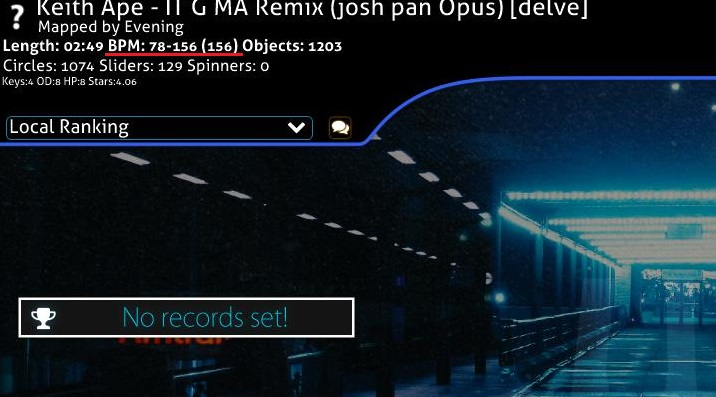
\includegraphics[width=\linewidth]{../part_3/imgs/normalize_img.jpg}
  \caption{Reference BPM Example}
  \label{fig:norm_ref}
\end{figure}
\subsection{Reference BPM}
You have seen this value a lot in this topic, but \textit{how} to do you get this value? The reference BPM is basically the value \textbf{in brackets} shown above.
In this case, simply \textbf{156}.

\subsubsection{Calculation of Reference BPM}
The Reference BPM is reliant on the longest duration mapped on a BPM. Hence, \textit{there is a possibility} that the Reference BPM will change, and you'll have to calculate all over again.

\subsubsection{Avoiding multiple Normalizations}
One way to do so is to litter the whole map with notes, \textbf{with intended breaks}, so that the game can process which reference BPM would be used, once you finished the whole chart.

The other would be to calculate manually, which is not recommended for complex cases.

\subsection{Tools for Normalization}
While you can just use these tools, it is important for you to understand this topic as a foundation to the next topics. \textbf{The tools can be found in the Annex}.
I'd recommend using Agka's SV tool over mine as it's more convenient.


